\documentclass[12pt, a4paper]{article}
\usepackage[utf8]{inputenc}
\usepackage{amsmath}
\usepackage{amsthm}
\usepackage{graphicx}
\usepackage{parskip}
\usepackage{hyperref}
\usepackage{fancyhdr}
\usepackage{lastpage}
\usepackage{tikz}
\usetikzlibrary{arrows,automata}

\title{Home work 6 - Solutions}
\author{Juan Pablo Royo Sales}
\date\today

\pagestyle{fancy}
\fancyhf{}
\fancyhead[C]{}
\fancyhead[R]{Juan Pablo Royo Sales - UPC MIRI}
\fancyhead[L]{RA - Homework 6}
\fancyfoot[L,C]{}
\fancyfoot[R]{Page \thepage{} of \pageref{LastPage}}
\renewcommand{\headrulewidth}{0.4pt}
\renewcommand{\footrulewidth}{0.4pt}

\begin{document}

\maketitle

\section{Exercise 29}
\subsection{Part a}

After step 33 we get the stationary distribution

\begin{align*}
P_{t \geq 33} = \begin{bmatrix}
  0.2346 & 0.3048 & 0.2631 & 0.1975\\
  0.2346 & 0.3048 & 0.2631 & 0.1975\\
  0.2346 & 0.3048 & 0.2631 & 0.1975\\
  0.2346 & 0.3048 & 0.2631 & 0.1975
\end{bmatrix}
\end{align*}

\subsection{Part b}

\begin{align*}
  P_{t = 32} = \begin{bmatrix}
    0.2346 & 0.3048 & 0.2631 & 0.1975\\
    0.2346 & 0.3048 & 0.2631 & 0.1975\\
    0.2346 & 0.3048 & 0.2631 & 0.1975\\
    0.2345 & 0.3048 & 0.2631 & 0.1976
  \end{bmatrix}
\end{align*}

Therefore the $P_{0,3}^{t=32} = 0.2631$

\subsection{Part c}
Given that

\begin{align*}
  P_{t \geq 128} = \begin{bmatrix}
    0.2346 & 0.3048 & 0.2631 & 0.1975\\
    0.2346 & 0.3048 & 0.2631 & 0.1975\\
    0.2346 & 0.3048 & 0.2631 & 0.1975\\
    0.2346 & 0.3048 & 0.2631 & 0.1975
  \end{bmatrix}
\end{align*}

Let $X$ be the state choosen u.a.r. at step 128

The $P_{0 \lor 1 \lor 2 \lor 3, 3}^{t=128} = 0.2631$ because to go the state $3$
no matter what initial state i choose is always that value.

\subsection{Part d}
In $t = 13$ we obtain that $\mid P_{0,i}^{t=13} - \pi_{i}^{*} \mid =
(0.0088,0.0047,0.0029,0.0071)$ which $max_i = 0.0088 < 0.01$

\section{Exercise 30}

Translating the problem to the following MC:

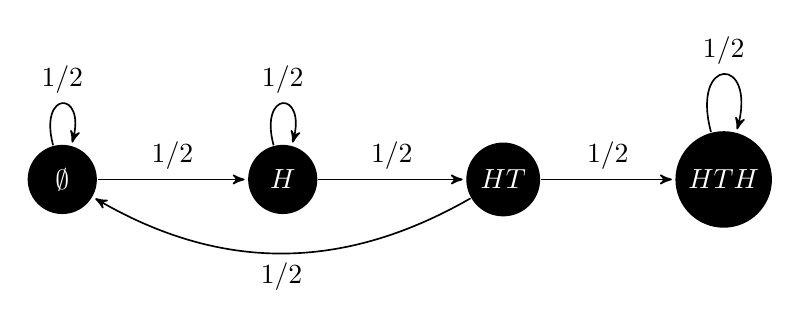
\begin{tikzpicture}[->,>=stealth',shorten >=1pt,auto,node distance=2.8cm,
  semithick]
  \tikzstyle{every state}=[fill=black,draw=none,text=white]

  \node[state] (A)              {$\emptyset$};
  \node[state]         (B) [right of=A] {$H$};
  \node[state]         (C) [right of=B] {$HT$};
  \node[state]         (D) [right of=C] {$HTH$};

  \path (A) edge [loop above] node {1/2} (A)
            edge              node {1/2} (B)
        (B) edge [loop above] node {1/2} (B)
            edge              node {1/2} (C)
        (C) edge              node {1/2} (D)
            edge [bend left]  node {1/2} (A)
        (D) edge [loop above] node {1/2} (D);
\end{tikzpicture}

Let $X_i$ be the expected number of steps starting from state $i$

We can calculate the Expected value:

\begin{align*}
  E[X_2] &= 1 + \frac{1}{2}E[X_0]\\
  E[X_1] &= 1 + \frac{1}{2}E[X_1] + \frac{1}{2}E[X_2]\\
  E[X_0] &= 1 + \frac{1}{2}E[X_0] + \frac{1}{2}E[X_1]
\end{align*}

Therefore replacing $E[X_0] = 10$

\section{Exercise 31}
\subsection{Part a}
\begin{itemize}
 \item It is \textbf{Aperiodic} because it contains loop
 \item It is \textbf{Irreducible} from the same reason as above 
\end{itemize}  

\subsection{Part b}
\begin{itemize}
\item It is \textbf{Aperiodic} because it contains loops
\item It is \textbf{Irreducible} because it is strongly connected
\end{itemize}  

\subsection{Part c}
\begin{itemize}
\item It is \textbf{Periodic} because it does not contains loops and there are
  periods of 2
\item It is \textbf{Irreducible} because it is strongly connected
\end{itemize}  

\subsection{Part d}
\begin{itemize}
\item It is \textbf{Aperiodic} because there is no way to form periods
  periods of 2
\item It is \textbf{Reducible} because if we go for example from $a$ to $c$
  there is no way to go back to $a$
\end{itemize}  

\subsection{Part e}
\begin{itemize}
\item It is \textbf{Aperiodic} because contains loops in $a$ and $b$ and in $c$
  although we can have a period with $b$ since we can go back to $a$ there is no
  period
\item It is \textbf{Irreducible} because it is strongly connected
\end{itemize}  


\section{Exercise 32}
\subsection{Part a}
Given a MC with states $S = \{i = 0, i = 1, i = 2, i = 3, i = 4\}$ where each
state $i$ represent the number of umbrellas we have in a place (home or office).

If $i = 1$ and it is raining then i take the umbrella, and if the destination
place i already have 3 umbrellas, then i will have 4 umbrellas.

\begin{align*}
  p_{1,4} = p
\end{align*}

because $p$ is the probability of rain. If $i=1$ but it doesnt rain i wont take
the umbrella, and in destination i will have 3 umbrellas not 4.

\begin{align*}
  p_{1,3} = 1 - p \equiv q
\end{align*}

Therefore we have the following diagrams.

\begin{tikzpicture}[->,>=stealth',shorten >=1pt,auto,node distance=2.8cm,
  semithick]
  \tikzstyle{every state}=[fill=black,draw=none,text=white]
    
  \node[state]         (A)              {$0$};
  \node[state]         (E) [right of=A] {$4$};
  \node[state]         (D) [right of=B] {$3$};
  \node[state]         (C) [right of=D] {$2$};
  \node[state]         (B) [right of=E] {$1$};

  \path
   (A) edge [bend right=-45] node {1} (E)
   (B) edge [bend left=45] node {p} (E)
   (B) edge [bend right=-45] node {q} (D)
   (C) edge [bend left=45]  node {p} (D)
   (C) edge [loop right] node {q} (C)
   (D) edge [bend left=45] node {q} (B)
   (D) edge [bend right=-45] node {p} (C)
   (E) edge [bend right=-45] node {p} (B)
   (E) edge [bend left=45] node {q} (A);
\end{tikzpicture}

Therefore we have the following stationary distribution

\begin{align*}
  \pi(2) = \pi(3) = \pi(1) = \pi(4)\\
  \pi(0) = \pi(4)q
\end{align*}

And also we know that,

\begin{align*}
  \sum_{i=0}^4 \pi(i) = 1
\end{align*}

Joining this last 2 equations we have,

\begin{align*}
  \pi(4)q + 4\pi(4) = 1
\end{align*}

and,

\begin{align*}
  \pi(4) = \frac{1}{q + 4} = \pi(1) = \pi(2) = \pi(3), \pi(0) = \frac{q}{q + 4}
\end{align*}

Therefore,

\begin{align*}
  P(getWet) = \pi(0) * p = \frac{qp}{q + 4}
\end{align*}

Having $p=0.6$ and $q=0.4$ then,

\begin{align*}
  P(getWet) \cong 0.0545
\end{align*}


\subsection{Part b}
For the probability to be less than 1\%, suppose that i need N umbrellas. Taking
the previous MC,

\begin{align*}
  \pi(N) = \pi(N-1) = \pi(N-2) = .... = \pi(1)\\
  \pi(0) = \pi(N)q
\end{align*}

\begin{align*}
  \pi(N) = \frac{1}{q + N} = \pi(N - 1) = ... = \pi(1), \pi(0) = \frac{q}{q + N}
\end{align*}

Therefore,

\begin{align*}
  P(getWet) = \frac{qp}{q + N}
\end{align*}

We want $P(getWet) = \frac{1}{100}$ or $q + N > 100pq$ then,

\begin{align*}
  N > 100pq - p = 100 * 0.4 * 0.6 - 0.4 = 23.6
\end{align*}

We need at least 24 umbrellas to reduce the probability to 1\%

\section{Exercise 33}
Given a MC with $n^2$ states of the form $(i,j) \in [1,n]^2$

Each node $(i,j)$ in MC is connected to $N(i)N(j)$ neighbors, where $N(i)$ denotes
the number of neighbors of state $i$ in the old Markov chain. Hence the number
of edges in the new chain comes to,

\begin{align*}
  2|E| = \sum_i\sum_j N((i,j)) = \sum_i\sum_j N(i)N(j) = \left( \sum_i N(i) \right) \left( \sum_j N(j)\right) = 4m^2
\end{align*}

If an edge exists between nodes $u = (i_1, j_1)$ and $v = (i_2, j_2)$ then
$h_{u,v} \leq 2|E|$

We need to show that for any node $(i,j)$, there exist a path of length $O(n)$
connecting to some other of the form $(v,v)$.

Since the graph is undirected, the cat can always go back to node $i$ in two
steps. At the same time, because the graph is connected, there is a path of length $k < n$ from $j$ to $i$. If $k$ is even, then the mouse will run into the cat. If $k$ is odd,
then the mouse will get to node $i$ when the cat is away. But since the chain is
non-bipartite, there must be a path of odd length from $i$ back to itself; let
the mouse follow this path, and it will run into the cat on the next return to
$i$. Thus the total length of this path from $(i, j)$ to $(i, i)$ is at most
$3n$. Each edge on this path requires at most $4m^2$ steps, thus the desired
upper bound on the time to collision is $O(m^2n)$ steps.

\section{Exercise 34}
\subsection{Part a}
Let $S$ be the satisfying assignment after $i$ steps be $A_i$
Let $X_i$ be the number of variables $A_i$ which match $S$. Therefor for $1 \leq
j \leq n - 1$,

\begin{align*}
  P[X_{i+1} = j + 1 \mid X_i = j] \geq 1/3\\
  P[X_{i+1} = j - 1 \mid X_i = j] \leq 2/3\\
\end{align*}

Using a MC $Y_0,Y_1, ...$ where $Y_0 = X_0$

\begin{align*}
  P[Y_{i+1} \mid Y_i = 0] = 1
  P[Y_{i+1} = j + 1 \mid Y_i = j] = 1/3\\
  P[Y_{i+1} = j - 1 \mid Y_i = j] = 2/3\\
\end{align*}


We let $h_j$ be the expected number of steps to reach $n$ when starting from $j$.

\begin{align*}
  h_n = 0\\
  h_0 = h_1 + 1\\
  h_j = \frac{2h_{j-1}}{3} + \frac{h_{j+1}}{3} + 1, 1 \leq j \leq n - 1
\end{align*}

Therefore

\begin{align*}
  h_j = 2^{n+2} - 2^{i+2} - 3(n - j)
\end{align*}

Then, $\Theta(2^n)$ steps.

\section{Exercise 36}
\subsection{Part a}

Lets assume that there are $k$ nodes in the sticky part, excluding $u$, and $k$
nodes in the ball part of the graph, including $u$, therefore the total number
of nodes are $n = 2k$. $h_{v,u}$ is the hitting time to reach the $k^{th}$ node
on a chain starting from $0$. For example $h_0$ in the chain of 2-SAT

\begin{align*}
  h_{v,u} = k^2
\end{align*}

$c_u$ is upper bounded by the expected time it takes travel to each of the
nodes in the clique and return to $u$.

\begin{align*}
  c_u \leq \sum_{w \in \text{clique}} h_{u,w} + h_{w,u} 
\end{align*}

Let $w$ and $x$ denote nodes in the clique other than $u$.
Let $i \in \{1,2,...k\}$ be the nodes on the stick, with 1 beings $u$'s neighbor
and $k$ being synonymous with $v$. So,

\begin{align*}
  h_{u,w} = \frac{1}{k}0 + \frac{k-2}{k}h_{x,w} + \frac{1}{k}h_{1,w} + 1\\
  h_{x,w} = \frac{1}{k}0 + \frac{k-23}{k-1}h_{x,w} + \frac{1}{k-1}h_{u,w} + 1\\
  h_{1,w} = \frac{1}{2}h_{u,w} + \frac{1}{2}h_{2,w} + 1\\
  h_{2,w} = \frac{1}{2}h_{1,w} + \frac{1}{2}h_{3,w} + 1\\
  ...\\
  h_{k-1,w} = \frac{1}{2}h_{k-2,w} + \frac{1}{2}h_{k,w} + 1\\
  h_{k,w} = \frac{1}{2}h_{k-1,w} + 1
\end{align*}

We obtain that $h_{k-i,w} + (2i + 1)$, and $h_{1,w} = h_{u,w} + 2k - 1$.
Replacing we get

\begin{align*}
  h_{u,w} = \frac{k^2 + 9k - 2}{2k}
\end{align*}

Using this,

\begin{align*}
  \frac{2|E|}{d(u)} = h_{u,u} = \frac{1}{d(u)} \sum_{w \in N(u)} (1 + h_{w,u})
\end{align*}

So replacing,

\begin{align*}
  \sum_{w \in N(u)} h_{w,u} = 2|E| - k = 2(k(k - 1) + k) - k = 2k^2 - k
\end{align*}

Therefore we have,

\begin{align*}
  c_u \leq \sum_{w \in clique} h_{u,w} + h_{w,u} \leq (k -1) \frac{k^2 + 9k - 2}{2k} + 2k^2 - k 
\end{align*}

Combining everything we get,

\begin{align*}
  h^2 = h_{v,u} \leq \text{ Cover time starting from } v \leq h_{v,u} + c_u = O(k^2) 
\end{align*}

Hence starting from $v$ cover is $\Theta(k^2) = \Theta(n^2)$

\subsection{Part b}
In previous section we showed that it takes time $\Theta(k^2)$ to cover the
clique part of the graph starting from $u$. We now show that $h_{u,v} =
\Theta(k^3)$, which gives us the required result. We can write down the
following system of equations, using the same node naming convention as before:

\begin{align*}
  h_{u,v} = \frac{k - 1}{k}h_{w,v} + \frac{1}{k}h_{1,v} + 1\\
  h_{w,v} = \frac{k - 2}{k - 1}h_{w,v} + \frac{1}{k - 1}h_{u,v} + 1\\
  h_{i,v} = \frac{1}{2}h_{i-1 ,v} + \frac{1}{2}h_{i+1,v} + 1
\end{align*}

We derive that $h_{w,v} = h_{u,v} + k - 1$ and $h_{k-i,v} =
\frac{i}{i+1}h_{k-i-1,v} + i$, and hence $h_{1,v} = k - 1kh_{u,v} + (k - 1)$. From this we get $h{u,v} = k^3$.

\end{document}
